\chapter{\label{cha:intro}Introduction}
%\addcontentsline{toc}{chapter}{Introduction}
% New title: Student translation quality: (norm-based) lingustic description and automatic estimation
% Learner translations: lingustic description and automatic quality estimation
% Human translation quality: translationese and distributional embeddings approaches
%
%\todo[inline]{(1) introduce a convention to refer to comparable originally authored texts in Russian as non-translation, a term first used in this meaning by~\cite{Chesterman2004}\\ (2) mention that all examples unless specifically marked come from our corpus, esp. RusLTC part of it}

\section{\label{sec:motivation}Motivation and Background}
% this section contextualises the problem and gives the rationale behind the research design
% aboutness and personal motivation
%My experience in translator education of many years led me to believe that translations, and student translations in particular, share specific features that make them recognisable as such. 
%Year after year, I annotated and commented the same suboptimal translation solutions. Their repetitiveness suggested that student translations can have automatically recognisable properties, which can be used to predict their quality. 

This thesis presents a comprehensive study of the relations between translationese and translation quality as captured by various assessment methods. 
%This thesis explores persistent properties of human translations in English-to-Russian language pair, testing the long-known and theoretically expected tendencies in translational behaviour as well as inferring new ones in a bottom-up manner. % new ones: I did not expect these to be among 28 shared translationese indicators amod/attrib, nnargs, wdlength, ccomp, pverbals, compar, fixed
It explores claims about translationese in English-to-Russian translation made in practical translation textbooks and arising from personal experience, and extends the existing scope of knowledge about the properties of translated language, making these properties even more visible to a professional eye. It often requires to know where to look to actually see. Raising awareness of the peculiarities of translated language can be useful in translator training, helping students to avoid typical pitfalls and recognise the cognitive constraints of the translation process. Importantly, this thesis investigates the extent to which translationese properties are taken into account in judgments about translation quality.
The originality and novelty of this study consists in testing the link between translationese and quality in a ML setup for the first time. 

% introduce the area of study
\paragraph{Area of study and rationale} 
%This research is set at the interface of empirical translation studies, corpus linguistics, computational linguistics and \gls{NLP}. Findings about linguistic properties of translated texts are based on experimental results obtained using machine learning techniques to predict quality labels and to reveal aspects of linguistic form that are objectively correlated with the available human judgments on translation quality. 

We draw from several research fields at various stages of this project trying to bridge the gap between theoretical translation studies and computational linguistics using supervised \gls{ML} methodologies. They can be roughly outlined as follows:
\begin{itemize}\compresslist{}
	\item translation quality related theories, including assessment approaches;
	\item empirical and computational translation studies focused on translationese research and studies on professionalism in translation;
	\item corpus linguistics focused on student translation and (register-)comparable corpora;
	\item machine translation quality research including human assessment methods and quality benchmarks;
	\item machine learning approaches to solve translationese-related and quality estimation tasks.
\end{itemize}

% contextualise the research, outline the current situation, introduce key terms
The specificity of translations in comparison with their sources and non-translated texts in the same target language register was acknowledged in literary criticism long ago. For example,~\citet{Berman1985} formulated 12 deforming tendencies in literary translation, including rationalisation (making text more coherent), ennoblement (more elegant style), destruction of underlying networks of signification, etc. However, it was not before Baker's seminal work~\cite{Baker1993} that translations and its linguistic properties became an object of study in their own right. After almost three decades of research, one of the central concepts in translation studies, \textit{translationese}, can be broadly defined as statistical deviations of translations from the expected target language norm, i.e. from language manifested in comparable originally-authored texts in the \gls{TL}. The body of research exploring peculiar regularities of translated language can be referred to as \textit{translationese studies}. 

From early works on, translationese was viewed as a strictly descriptive, non-evaluative term reflecting the nature of translation~\cite{Gellerstam1986, Baker1993}. It was established that all translations are inevitably different from comparable originally-authored texts. It does not mean that translated texts are written to a lower professional standard than comparable non-translations~\cite{Sutter2017}. Instead, they form their own language subsystem and can be approached as a language variety.

% why do this research?
% why the proposed approach is feasible
% hypothesis
At the same time, the amount and type of translationese observed in translations can be indicative of translation quality. For translation scholars and educators, professionalism in translation is often associated with the ability to identify translation problems and find the more acceptable solution for them~\cite{Pym2003}, i.e., most importantly, to be able to recognise and counteract the natural gravitational pull of the \gls{SL} which triggers literal renditions.

The association between the amount of translationese and translation quality was either assumed or demonstrated in a number of publications, such as~\citet{Scarpa2006, Rabadan2009, Sutter2017} as well as in~\citet{Loock2013, Loock2016}~\cite[as quoted by][]{Sutter2017}. For example,~\citet{Scarpa2006} found that simplification correlated with lower-scoring translations and explicitation correlated with higher quality scores. \citet{Sutter2017} interpreted the distance between individual student translations and comparable professional texts in scatter plots as indicative of lower quality. They also found statistical differences between student and professional translations in a univariate analysis on a number of language-independent easily-extractable features in English-to-French translation of fiction and in French-to-Dutch news. Our own early univariate exploration of student translations indicated that they were more distant from the reference corpus than professional translations on a number of linguistically-motivated features~\cite{Kunilovskaya2018profiles}.

% establish a niche, identify the gap
Despite \textit{translationese studies} is an established research direction in the empirical translation studies, the applicability of translationese features to \gls{HTQE} remains unclear. It is especially surprising, given that translationese-based approach was used in a much more dynamic and technologically advanced area of \gls{MTQE}~\cite{Aharoni2015} and in the machine translation detection task~\cite{Carter2012}. In particular, \citet{Aharoni2015} showed that the higher the translationese classification accuracy (i.e. the better machine translations were distinguished from non-translations), the lower the expected translation quality. \citet{Aranberri2020} also found translationese predictive of~\gls{MT} quality. Interestingly, \citet{Rubino2016} used surprisal and distortion measures derived from delexicalised language models, which they refer to as quality estimation indicators, to discriminate between novice and professional translations.
Nonetheless, we are not aware of any empirical studies that explore the suggested feasibility of a translationese-based human translation quality model. %, except our own previous work~\cite{Kunilovskaya2019qua, Kunilovskaya2020vars}.

\paragraph{Hypothesis} Thus, this research is designed to test a hypothesis that translationese indicators could be predictive of human translation quality. This hypothesis will be confirmed if we find that lower-ranking translations exhibit stronger translationese tendencies than their higher-ranking counterparts, and if a ML algorithm built to predict quality labels/scores returns a reasonably high performance compared to alternative representations.  

Generally, this research contributes to a fairly new research area of automatic prediction of human translation quality. The term \gls{HTQE} seems to have first appeared in a PhD thesis by~\citet{Yuan2018} and a subsequent publication by the same author~\cite{Yuan2020}. In their work, the concept of quality estimation for~\gls*{MT} is adopted to predict English-to-Chinese human translation quality. 
The alternative automatic approach to MT quality (quality evaluation) measures deviations from a MT candidate and human reference translations. It is hardly applicable to human translation, even theoretically, due to a wide range of legitimate variation in linguistic expression that translators can resort to. In human translation, it seems unfair to penalise renditions because they deviate from a pre-selected good translation.
In another research on HTQE, known to us, \citet{Zhou2019} formulated the task of predicting human translation quality as an unsupervised graph matching problem. They employ cross-lingual word embeddings to represent sources and targets, and measured the distance between respective vectors, reporting Spearman 0.529 for their Japanese-to-English data. 

%\todo[inline]{We did the same in a supervised setting on self-trained cross-lingual projection (MUSE) achieving the best result on binary quality labels of macro F1-score = 63.0, the current result on our focused representation is 61.40, with the chance level of 51.63. Shall I report that?}
Other attempts to develop automatic approach to measure human translation quality were not formulated as a ML task, but present corpus-based studies and observations. \citet{Sutter2017} report results of a multifactorial corpus analysis backed with \gls{PCA}-based visualisation to give a translation teacher a method to `objectify formative quality assessment' (p.25). They perform monolingual comparison, presenting student translations against the backdrop of comparable professional translations and non-translations as two possible TL norms, and reducing the concept of human translation quality to its acceptability aspect, i.e. to the TL quality. 

% disadvantages of the proposed approach
\paragraph{Anticipated issues and challenges} We envisage a few theoretical and practical challenges that should be kept in mind. This paragraph discusses caveats that limit the scope of this research and possible contingency measures to curb their effects on the outcomes. 
One limitation of a translationese-based approach to translation quality estimation is that it reflects only one of translation quality aspects, namely, fluency (also referred to as acceptability/readability). It does not have access of the semantic relation between source and target texts, known as the accuracy/adequacy aspect of translation. Nonetheless, as it is shown in Sections~\ref{sec:feats4qua} and~\ref{ssec:bin}, there are good reasons to believe that 
\begin{itemize}\compresslist{}
	\item translationese-related fluency might have a large impact on human perception (`It does not sound right' reaction),
	\item fluency and accuracy might be difficult distinguish in an annotation task, 
	\item fluency and accuracy might correlate to a great extent -- it is difficult to imagine a human translation produced in good faith that is very fluent but inaccurate; inaccuracies usually render translated text less readable and coherent than expected and are rarely seamless,
	\item differences between student and professional translations are mostly related to the fluency aspect of translation quality.
\end{itemize}

Frequency-based translationese features are not immune to sparsity. At sentence-level, where the observations are short, many features can have zero values. Therefore, the proposed features, especially from the morphosyntactic feature set, are better suited for document-level experiments.
%provided that the documents are of suitable lengths (typically, of at least 450 words; the studies that use chunking usually limit their text fragments by 2000 tokens).

Assessing translations on the basis of translationese indicators, requires carefully selected external resources that would represent the expected standard, i.e. either comparable professional translations, or reference texts, or both. It is not uncommon to collect and maintain such resources in both educational~\citep{Bowker2001} and industrial settings (translation memories and \gls*{TL} reference corpora)~\citep{Massey2019}, but such resources can be less available in other circumstances. 
Constructing a comparable corpus of non-translations to represent \gls*{TL} textual fit~\citep{Chesterman2004} is one of the challenges in this project. Register of the source and translational conventions associated with it are known to be one of the major factors shaping linguistic properties of translations~\cite{Lapshinova2017}. A preliminary step in this research was to design an approach to select a subset of non-translations from a large TL corpus that would be functionally-comparable to the English source texts in the parallel subcorpora~\cite{Kunilovskaya2019crossling}.

By design, this research is focused on shining-through form of translationese. Some researchers express reservations whether SL-induced translationese can explain all specificity of translations. They name other factors that might be at work, including translators' awareness of their sociocultural roles and positions, i.e. translation norms~\cite{Laviosa2008, Delaere2012}, extralinguistic conditions of the translation situation such as time constrains and perceived responsibility, rather than lack of professionalism and inadequate language use. It is necessary to control for some of these other factors in the experiment design by selecting register-homogeneous translations produced under similar communicative and translation conditions by many subjects of known professional status.

%application, practical relevance
% low-risk taking examination scoring and autonomous learning feedback
\paragraph{Practical relevance} This thesis primarily contributes to the understanding of translationese and its relation to quality judgments. Our results can be used as a module in a \gls{HTQE} tool to estimate translation quality with regard to the amount of translationese manifested it a translated document. There is a number of potential use cases for \gls*{HTQE}, primarily in education, certification and quality control.

Probably the largest sphere where there is a wide need to score human translations is translator education and language learning scenarios. Translation programmes of various standing (university degrees in translation, vocational training courses or advanced professional development programmes) as well as practical translation courses included in the foreign language education programmes routinely grade students' written submissions. Some form of summative assessment is indispensable in test and exam settings. However, although institutional grading manuals can be very detailed, translation quality assessment often proceeds ``according to the lordly, but completely unexplained, whimsy of `It doesn't sound right.''', a much quoted and accurate description offered by~\citet[p. 142]{Fawcett1981}. An automated approach can make this process more objective and systematic, devoid of personal preferences and expectations, more uniform in terms of rigour, and immune to the known negative effects common for all human evaluation, including lapses of concentration and the order of translations to be graded~\cite{MinacoriVibert2010}.    

A reliable automation of the scoring process can help to better monitor translation students' progress and provide qualitative feedback on their work more often. It is true that getting regular formative human feedback on their course work between the tests would be more useful, but, given the class sizes and the enormous effort required to assess translations manually, it is unavailable in many translation programmes.
Automatic feedback can also contribute to self-evaluation and independent learning. 

Apart from qualification exams in the training environments, many countries have certification requirements that facilitate the access to professional jobs. Certification usually includes a translation task, which is scored by several trained evaluators. In the context of the \gls{ATA}, there is a points-based threshold (more than 46) after which the error annotation can be abandoned because the translation is obviously below the expected quality standard\wlvfootnote{see the instructions at \url{www.atanet.org/certification/Framework_2017.pdf}}. An automatic scoring algorithm can be used as a preliminary filter to identify the submissions that can be desk-rejected for being significantly below the standard. A similar functionality can be useful for filtering out very poor submissions to translation contests to help a human jury focus on, for example, the top 30\% of the participants to identify the winners. 

In the industrial contexts, an automatic scoring tool for human translations can be applied on both the language service provider side for internal quality control purposes or on the customer side for ensuring the quality of a translation obtained from a translator or a translation agency, possibly as an extension of Translation Quality Assurance procedures, if they are available. It can be especially useful if a translation user does not possess a bilingual competence and does not want to involve a third party for a linguistic expertise. A similar need for a quick and cheap evaluation of translation quality arises when several human translations of the same sample are available and the customer is seeking to detect the best of them. 

\section{\label{sec:task}Research Aim and Objectives}
% overarching purpose of a research project
% two main aspects: linguistic(!) features and four labels: comparison to other representations and extension to doc- and sent-level is implied
This thesis sets out to explore the performance of translationese indicators inspired by contrastive linguistics and translation studies in the task of predicting a range of human translation quality judgments.

To achieve this overarching purpose, we define a number of research objectives:
\begin{enumerate}\compresslist{}
	\item Develop a set of translationese indicators motivated by previous findings in translationese studies and contrastive analysis for English-to-Russian language pair (mass-media register).
	\item Test the proposed feature sets in a translation detection task (translationese classification) on two competence-based varieties (student and professional translations). This objective includes:
	\begin{enumerate}[(a)]\compresslist{}
		\item building a motivated comparable corpus of non-translations, the second class in the translationese-diagnostic binary classification (translations vs. non-translations); 
		\item comparing the performance of proposed feature sets to each other and to alternative representations, including multilingual/cross-lingual embeddings;
		\item identifying and describing strong translationese indicators.
	\end{enumerate}
	\item Collect various types of human quality judgments. This involves a number of preliminary steps:
	\begin{enumerate}[(a)]
		\item explore the approaches to produce quality labels in human and machine translation applicable to our data;
		\item build a parallel corpus of professional translations and generate a reasonably diverse subset of student translation from an existing \gls{LTC} to represent experience-based categories as a proxy for quality;
		\item produce quality labels from existing \gls{RusLTC} `grade' attribute and continuous document- and sentence-level scores from existing error annotation.
		\item set up a direct assessment annotation experiment and produce respective document- and sentence-level scores.
	\end{enumerate} 
	\item Explore alternative approaches to text representation for document- and sentence-level quality estimation tasks. More specifically:
	\begin{enumerate}[(a)]
		\item use \textit{tf-idf} as a simple baseline,
		\item generate alternative explicit features designed for \gls*{MTQE} within QuEst++ framework, 
%		\item learn a cross-lingual distributed representation model on a register comparable corpus and use word embeddings from it, as suggested in \citet{Yuan2018,Zhou2019};
		\item apply cross-lingual sentence encoders, fine-tuned on \gls{STS} task and on DA scores in a \gls*{MTQE} task, % including \textit{TransQuest} \cite{Ranasinghe2021},
		\item generate representation from state-of-the-art general-purpose contextualised word embedding models: a dedicated Russian language model and a multilingual \textit{mdeberta3-base}.
%\todo[inline]{+ explore the possibility of combining translationese and bilingual approaches for better coverage of both fluency and accuracy aspects of quality.}
	\end{enumerate} 
	\item Compare the outcomes of classification and regression experiments, supported by feature analysis where possible, across various representations and types of quality judgments.
	% combining translationese-based approach to capturing fluency, the major problem with advanced learners translations (if the two aspects of translation quality are to be distinguished), and accuracy-oriented bilingual features and embeddings from Sentence Transformer-based models seems difficult because translationese approaches operate on the document-level, while deep-learning models are limited to short segments. Actually, the average student translation document length is within the the range that is manageable by Bert (450 tokens and 512 tokens, respectively)  
\end{enumerate}

% outline of the research design/methodology and how are we going to address the limitations
\section{\label{ssec:design}Research Design} 
This research focuses two components of a quality estimation task: types of quality labels/scores and text representations. We do not lay much emphasis on the learning algorithm and use a simple \gls{SVM} with default settings. For ML quality control, i.e. to ensure that SVM returns a reasonable performance on our tasks, we implemented a one-layer neural model.

\paragraph{Quality labels} One of the important questions that we explore in this thesis is generating translation quality benchmarks, i.e. sets of gold-standard labels/scores reflecting human judgments about translation quality that can be used as learning targets in a ML setup. 
Weak artificial intelligence, as a research and engineering domain, seeks to teach the machine to solve tasks that can be performed by humans. 
%Recent advances in neural networks demonstrate that there are fewer and fewer tasks that are exclusively human and are inaccessible to machines. 
For now, judging human translation quality is perceived as one of the tasks that is challenging for the machines. It is not entirely because it requires unstructured professional knowledge to yield to automation. It is also because translation quality is difficult to capture in a reliable way due to the notorious subjectivity of the underlying concept. This thesis compares the performance of various document representations, including translationese indicators, on labels/scores from several methods to annotate human translations for quality. These experiments can reveal dissimilarities between assessment methods with regard to the type of quality they capture. 
%However, in our experience, a professional jury in a translation contest usually agrees on the top and, especially, on bottom, translations (with possible fine-grained disagreements).   
Our experiments are run on the four types of quality categories/judgments:
\begin{enumerate}\compresslist{}
	%	\setlength{\itemsep}{0.5pt}
	\item Binary quality: coarse-grained binary quality labels, derived from holistic document-level assessment of exam translations in several Russian universities and of submissions to a number of translation competitions;
	\item Professionalism: ontological status of texts based on the meta information about translators;
	\item Scores from error annotation: aggregated measures of quality based on error statistics;
	\item Scores from direct assessment: a mean score across two annotators.
\end{enumerate}

Annotated student translations come from an existing multi-parallel \gls{LTC} which, inter alia, collects quality assessment carried out in real-life contexts (student translation competitions, graded exam translations, error annotation as part of the formative feedback). The quality judgments were produced outside of a well-controlled -- and artificial -- experimental setup.
This explains the lack of all four labels for all student translations in our research corpus. Instead, we have multiple intersecting subsets shown in Figure~\ref{fig:subsets}. We tried to acquire as much corpus data for each type of assessment as possible without compromising the integrity of the categories.
\label{pg:subsets}
\begin{figure}[h ] % htbp
	\centering
	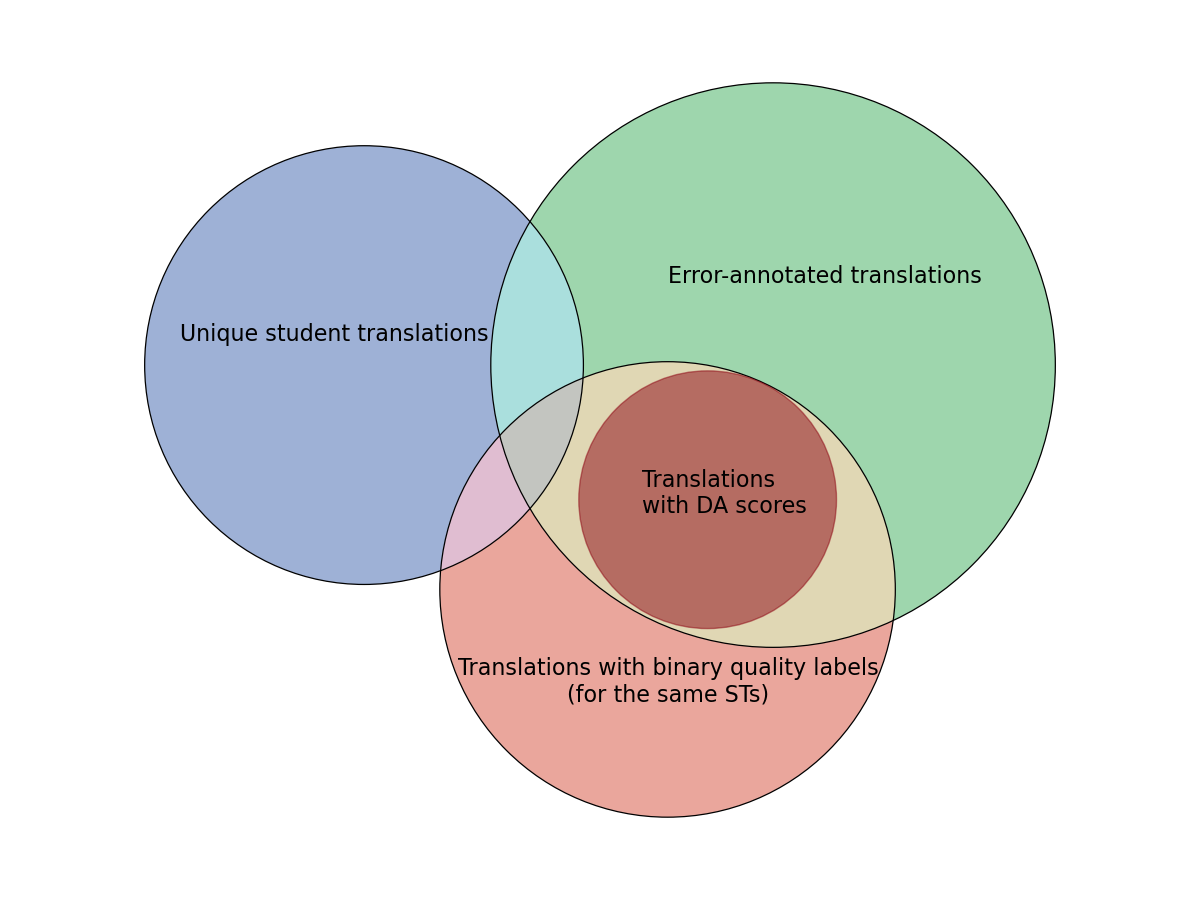
\includegraphics[scale=0.5]{figures/subsets}
	\caption{Size of student translations subsets with various types of quality judgments (number of sources, number of targets, number of aligned sentences)}
	\label{fig:subsets}
\end{figure}

%\wlvfig[0.5]{subsets}{Size of student translations subsets with various types of quality judgments (number of sources, number of targets, total number of translated sentences)}

A detailed description of how each subset was selected can be found in Section~\ref{ssec:subsets}; the annotation setups and associated reliability studies appear in Section~\ref{sec:mygold}. 

\paragraph{Features and representations} In this thesis the performance of several sets of well-established and novel language-pair specific translationese indicators is thrown into perspective of bilingual features from \textit{QuEst++}\wlvfootnote{\url{github.com/ghpaetzold/questplusplus}}, a translation quality estimation framework for~\gls*{MT}~\cite{Specia2015quest}, and a number of contextualised embedding models.

Traditionally, the explorations of translationese are based on manually-selected explicit features that capture a particular phenomenon represented by its normalised frequency. Probably the most popular feature set of diverse and elaborate hand-engineered features was proposed by~\citet{Volansky2012}, and later extended by~\citet{Sominsky2019}.
In the last decade, the research paradigms in translationese studies shifted from univariate statistical analyses to supervised and unsupervised \gls*{ML} methods, which take into account feature combinations. A standard practice is a bottom-up approach which includes as many features as possible and empirically establishes their effectiveness through feature selection~\cite{Evert2017, Yuan2018}. 
% which has been around since Baroni and Bernardini's~\citeyear{Baroni2005} experiments on professional English-to-Italian translations has made a comeback quite recently~\cite{Chowdhury2020,Chowdhury2021}. 
An alternative approach consists in producing sparse or dense document vectors from sequences of items in that document. Vectorisers were run on character, word or \gls{PoS} n-grams~\cite{Popescu2011,Baroni2005,Carter2012,Eetemadi2015,Rabinovich2017,Lapshinova2019}. %, because it helped with sparsity and domain differences between translations and non-translations. 
%  that retain functional words while convert other words to \gls*{PoS}
More recent studies make use of language modelling approaches (i) to measure entropy/perplexity of a model trained on non-translations and run on translations~\citep{Karakanta2019,Nikolaev2020}; or (ii) to generate static embeddings for \gls*{PoS} or semantic tags sequences in translated and non-translated corpora~\citep{Chowdhury2020,Chowdhury2021}. 

This thesis compares the performance of explicit linguistically-motivated features against representations from a number of embedding models, which are supposed to capture various properties of translations. 
The rationale behind using embeddings is that these representations might capture complex non-local syntactic and semantic information that is difficult to encode manually. Neural representations are expected to perform better than hand-engineered features, but relative ease of generating embeddings and expected superior performance come at the expense of explainability. 
%At the same time \citet{Yuan2018} results demonstrated that the power of neural models might be overestimated on the challenging task of \textit{HTQE}.    
At the moment there is no published work on translationese (or HTQE) using recent contextualised embedding models, except~\citet{Pylypenko2021}. In this thesis, we compare the performance of hand-crafted translationese indicators and document-averaged embeddings to solve the tasks of translation detection and HTQE. 

Although this research is based on human translations, we make a point of exploring theoretical and practical approaches used in \gls*{MTQE}. We are aware of the ontological differences that make these two translation varieties very dissimilar, but we hope that there can be a productive interconnection between the two closely related research areas: machine translation quality estimation and quality assessment in translation studies. 
We see it as part of our task to reveal the opportunities for mutually beneficial cooperation between machine translation and translation studies. Given our primary focus on student translations, we are mostly interested in borrowing from MT approaches to solve our task. At the same time, the increased quality of MT, especially with regard to fluency, makes the task of MTQE more demanding in terms of ability to reveal fine-grained quality distinctions.
Besides, MT paradigm can benefit from shifting to document level, which is the default setting in translation studies, and is called for in MT, especially when comparing its performance to human translators~\citep{Laubli2018,Voita2019}.

The particulars of a research design depend on the desired trade-off between interpretability, scalability and performance, among other factors. Our preferences and interests are more on the translation studies side: we use ML methods to understand the nature of translationese better and to produce interpretable automatic quality predictions, if possible. Previous research returned mixed results on language-independent generic features~\citep{Sutter2017}. Some researchers found that language-specific indicators return better results in translationese studies~\citep{Hu2021}. We are prepared to sacrifice some scalability of the approach for higher explaining power, validity and diagnostic potential. To this end, we engineer features, based on theoretical or empirical evidence from translation studies or contrastive linguistics for a given translation direction. The embeddings are used in this thesis for quality control to throw our feature-based models into perspective of the achievable for each type of labels/scores. 

\paragraph{Document- vs sentence-level} This research is focused on the document-level scenario as it is more in line with the nature of human translation. In most real-life scenarios, human translation evaluation is required at document level. 
However, it can be helpful if an algorithm could highlight segments that might require reworking or additional editing due to being inaccurate with regard to the source or due to being overtly translational at the level of expression. Besides, sentence- or segment-level predictions are more compatible with neural models. \textit{Longformer} approaches~\cite{Beltagy2020} are still in the making and are not available for Russian at the time of writing, and we had to rely on aggregation of sentence vectors via mean-pooling to obtain document representations, which might be a crude simplification.

Our experiments are framed as text classification/regression problems solved with the default linear-kernel \gls{SVM} (and a simple one-layer neural model for comparison). The classification results, including those after feature selection, are complemented with feature analysis, which traces the performance of prominent translationese indicators and their groups in quality estimation experiments.

\section{\label{sec:contributions}Main Contributions}

The main contributions of this PhD thesis are as follows: 

\begin{itemize}\compresslist{}	
	\item It proposes a theoretically-motivated feature set for translationese diagnostics in English-to-Russian translation. Its applicability to other language pairs (with adaptation) and registers has been tested in other projects, but these results are outside the scope of this thesis.
	
	\item We revealed strong translationese indicators, which were mostly associated with the \textit{shining-through} trend in translational behaviour, and demonstrated that lower-ranking translations exhibited more translationese than higher-ranking translations.  
	
	\item This study showed that morphosyntactic translationese indicators were competitive against QuEst++ features and some distributed representations, at least on document-level labels from holistic assessment. 
	
	\item It was shown that distinctions between professional and student translations were less related to translationese than expected. Professional translators might be better at recognising and counteracting some influences of the ST, but they generate other types of translationese which makes them easy to distinguish from non-translations. If anything, professional translations were more homogeneous than student translations, probably due to a more standard repertoire of translation solutions. 
	
	\item The experiments revealed dissimilarities between three quality assessment methods in terms of sensitivity to translationese and in terms of capturing document-level properties. Document-level holistic assessment was most translationese-aware, error-based scores demonstrated some alignment with translationese properties of texts and performed better at document-level. Scores from direct assessment returned better results at sentence level and were largely agnostic of translationese. 
	
	\item We released datasets for document- and sentence-level \gls{HTQE} experiments in English-to-Russian language pair with three types of quality judgments\wlvfootnote{The datasets are available from the RusLTC website: \url{www.rus-ltc.org/static/html/about.html}}. First, there is a dataset with document labels, including 360 parallel documents with good/bad labels, 738 documents with professional/student labels and 497 comparable documents originally-authored in Russian. Second, there are datasets with document- and sentence-level continuous quality scores from error annotation and from Direct Assessment experiment (553 documents/12,369 sentences with error-based scores, including 140 documents/3,224 sentences annotated in DA setup).

\end{itemize}

\section{\label{sec:papers}Publications}
%\todo[inline]{comment on the contribution of each publication to various parts of the thesis, reduce the list to only directly relevant}
Preliminary results related to the ideas developed in this thesis appeared in the following publications:
\begin{enumerate}\compresslist{}
	\item Kunilovskaya, M. and Sharoff, S. (2019) `Towards functionally similar corpus resources for translation', \textit{Proceedings of Recent Advances in Natural Language Processing}, Varna, 2-4 September, pp. 583–592, doi: \url{10.26615/978-954-452-056-4\_069}.
	\item Kunilovskaya, M., Taslimipoor, S. and Ilyushchenya, T. (2019) `Functional text representations for building cross-linguistic comparable corpora in English and Russian', \textit{Proceedings of 12th Workshop on Building and Using Comparable Corpora (BUCC 2019)}, Varna, 5 September, pp. 37--45. Available at: \url{comparable.limsi.fr/bucc2019/Kunilovskaya\_BUCC2019\_paper5.pdf} (Accessed: 16 June 2022).
	\item Kunilovskaya, M. and Lapshinova-Koltunski, E. (2019) `Translationese features as indicators of quality in English-Russian human translation', \textit{Proceedings of the 2nd Workshop on Human-Informed Translation and Interpreting Technology (HiT-IT 2019)} (pp. 47–56), Varna, 5-6 September, doi: \url{10.26615/issn.2683-0078.2019\_006}.
	\item Kunilovskaya, M. and Lapshinova-Koltunski, E. (2020) `Lexicogrammatic translationese across two targets and competence levels', \textit{Proceedings of the 12th Conference on Language Resources and Evaluation}, Marseille (online), 13--15 June, pp. 4102–4112. Available at: \url{aclanthology.org/2020.lrec-1.505} (Accessed: 16 June 2022).
	\item Kunilovskaya, M. and G. Corpas Pastor (2021) `Translationese and register variation in English-to-Russian professional translation', in Lim, L. and  Li, D. and Wang, V. (eds.) \textit{New Perspectives on Corpus Translation Studies}. Singapore: Springer, pp. 133--180, doi: \url{10.1007/978-981-16-4918-9\_6}.
	\item Kunilovskaya, M., Ilyushchenya, T., Morgoun, N. and Mitkov, R. (2021) `Source language difficulties in learner translation: evidence from an error-annotated corpus', \textit{Target}, doi: \url{10.1075/target.20189.kun}. 
	\item Kunilovskaya, M., Lapshinova-Koltunski, E. and Mitkov, R. (2021) `Translationese in Russian literary texts', \textit{Proceedings of the 5th Joint SIGHUM Workshop on Computational Linguistics for Cultural Heritage, Social Sciences, Humanities and Literature at EMNLP}, Punta Cana (online), 11 November, pp. 101--112, doi: \url{10.18653/v1/2021.latechclfl-1.12}.
\end{enumerate}

Some of these papers report results for similar experimental setups. However, the results reported in this thesis are based on a fresh run of these experiments after we had addressed the issues identified in preliminary studies. 

\section{\label{sec:structure}Thesis Structure}

Chapters~\ref{cha:indicators}-\ref{cha:quest} discuss previous research relevant for each project's task and describe proposed solutions. Chapters~\ref{cha:translationese}-\ref{cha:pro_qua} describe the experimental setup, report and analyse the outcomes of the experiments. 

% Translationese studies and features; relevance fot QE
Chapter~\ref{cha:indicators} introduces translationese studies, a research direction within empirical translation studies, which describes and explains linguistic properties of translations. We provide the main theoretical underpinnings of our research hypothesis, showing the link between translationese and translation quality. The last part of the chapter gives an overview of the proposed feature sets along with the extraction procedures. We also explain the rationale behind feature selection, using existing empirical evidence and approaches to translation detection.
 
% LTC, competence as a proxy for quality,  comparable corpora; textual data
Chapter~\ref{cha:varieties} discusses previous research on differences between competence-based (professional) varieties of translated language (student and professional translations), which are often interpreted as a proxy for quality. This includes a brief overview of learner translator corpora as a common source of human quality-annotated translations.
A separate paragraph deals with theoretical and practical issues of building cross-linguistically comparable corpora for translationese research.  
The second part of the chapter gives more details on the sources and nature of the textual data in this research. It presents the rationale for subsetting student translations from an existing \gls{LTC}. The description of textual data, including large external resources required for feature extraction, is complete with quantitative parameters and preprocessing details.

% Translation quality methods and best benchmarking practices applied to our textual data
Chapter~\ref{cha:quest} compares MT and \gls{HT} in the context of quality: we give a concise overview of the main theoretical aspects of translation quality and summarise approaches to quality estimation, including previous research in \gls{HTQE}. The chapter focuses text representations for QE task, highlighting the more prominent feature-based and embedding-based solutions. The second part of the chapter overviews established practices and recommendations to produce manual `gold standards' for ML experiments modelling translation quality. Importantly, Chapter~\ref{cha:quest} contains a description and results of cross-annotation, error annotation and direct assessment experiments, which yielded quality labels/scores used in this thesis.

Chapter~\ref{cha:translationese} presents the results of translationese classifications. We compare the performance of a number of representations on professional and student translations. A considerable part of the chapter is given to feature analysis using automatic feature selection and univariate correlation and statistical significance testing. It allows us to identify strong translationese indicators in English-to-Russian translation of mass-media texts.

Chapter~\ref{cha:pro_qua} is our main experimental chapter. It opens with classification results on professionalism labels and binary quality labels. Section~\ref{sec:_scores} reports regression outcomes for error-based and DA scores. The experiments are run at document and sentence levels. The results at document level are backed up by feature analysis. 

% Conclusion
Chapter~\ref{cha:fin} summarises our findings and draws conclusions by chapter. We discuss limitations and possible directions for future work. 